\documentclass[12pt]{report}

\usepackage{geometry}
\usepackage{tabu}
\usepackage{dirtytalk}
\usepackage{graphicx}
\usepackage{url}
\usepackage{float}
\usepackage{listings}
\usepackage{algpseudocode}
\usepackage{algorithm}
\usepackage{algorithmicx}
\usepackage{subcaption}
\usepackage{verbatim}
\usepackage{amsmath}
\usepackage{wrapfig}
\usepackage{color}

\usepackage{amsthm}
\usepackage{verbatimbox}
\usepackage{multicol}
\usepackage[titletoc,title]{appendix}
\usepackage{amsfonts}
\usepackage[font={it}]{caption}
\usepackage{afterpage}
\usepackage{caption}
\usepackage{lipsum}
\usepackage{csquotes}
\usepackage{fancyvrb}

\usepackage{lmodern}

% For citing and referencing.
\usepackage{natbib}
\newcommand{\citebu}[1]{(\citeauthor{#1} \citeyear{#1})}
\newcommand{\citediagram}[2]{(\citeauthor{#1} \citeyear{#1}, p.#2)}
\newcommand{\citesoftware}[1]{(\citeauthor{#1} \citeyear{#1})}

\newcommand{\figurewidth}{0.6\textwidth}
\newcommand{\imagewidth}{0.5\textwidth}

\newcommand{\quotebu}[1]
{
  \begin{displayquote}
    \textit{#1}
  \end{displayquote}
}

\geometry{
  a4paper,
  total={170mm,257mm},
  left=30mm,
  right=30mm,
  top=20mm,
  bottom=30mm,
}

\pagenumbering{roman}

\theoremstyle{definition}
\newtheorem{definition}{Definition}[section]

\begin{document}

  \renewcommand{\familydefault}{\sfdefault}
  \fontfamily{lmss}\selectfont

  \begin{titlepage}
    \centering
    {\Huge Bournemouth University\par}
    \vspace{0.5cm}
    {\Large National Centre for Computer Animation\par}
    \vspace{0.5cm}
    {\Large MSc in Computer Animation and Visual Effects\par}
    \vspace{5cm}
    {\huge \bfseries evulkan\par}
    \vspace{0.5cm}
    {\Large \bfseries \textit{A Vulkan Library}\par}
    \vspace{2cm}
    {\Large Eimear Crotty\par}
    % \includegraphics[width=0.15\textwidth]{images/MIT.png}\par\vspace{1cm}
    \vfill
    {\Large August 2020}
  \end{titlepage}

  \chapter*{Abstract}
    Vulkan is a low-level graphics API which aims to provide users with faster
    draw speeds by removing overhead from the driver. The user is expected to
    explicitly provide the details previously generated by the driver. The
    resulting extra code can be difficult to understand and taxing to write
    for beginners, leading to the need for a helper library.

  \chapter*{Acknowledgements}

    \vspace{1cm}
    Jon Macey\\
    Mum, Dad, Rory, Aisling, Aoife, Ellie.\\
    Neil.
    % TODO.

  \chapter*{Dedication}

    %TODO

  \tableofcontents

  \listoffigures

  \chapter{Introduction}
    \pagenumbering{arabic}
    Vulkan \citesoftware{vulkan} is a cross-platform graphics and compute API.
    It aims to provide higher efficiency than other current
    cross-platform APIs, by using the full performance available in today's
    largely-multithreaded machines. Vulkan achieves this by allowing tasks to be
    generated and submitted to the GPU in parallel (multithreaded programming).
    In addition, the API itself is written at a lower-level than other graphics
    APIs, meaning that the developer is required to provide many of the details
    previously generated by the driver at run-time.\\

    This project aims to alleviate this cost by providing a wrapper library for
    Vulkan, which allows a developer to use some of the more common features of
    Vulkan with much less effort than writing an application from scratch. This
    library is written in C++, using modern C++ features, adheres to both the
    official C++ Core Guidelines and Google C++ Style Guide and is fully unit
    tested. The library is available for download from GitHub and can be built
    using CMake.\\

    The library is specifically written with beginners and casual users of
    Vulkan in mind. The examples included in the repository provide a
    demonstration of how to use the library for different purposes, including
    drawing a triangle, loading an OBJ with a texture and using multiple passes
    to render simple objects with deferred shading. A non-goal is to create a
    library which is as fast as writing pure Vulkan, however the library
    must be reasonably fast.\\

  \chapter{Previous Work}

    While Vulkan is a relatively new API for graphics and compute, many engines
    now support Vulkan, including CryEngine, Valve's Source, Unity and Unreal
    Engine. As a result, there are many libraries and utilities available
    online for Vulkan, each of which serves a different purpose.

    \section{V-EZ}

      AMD created the open-source V-EZ library \citesoftware{vez}. Its main goal is to increase the
      adoption of Vulkan in the games industry by reducing the complexity of
      Vulkan. It is a lightweight C API wrapped around the basic Vulkan API.
      It is part of the GPU-Open initiative. \\
      
      It still requires the user to have a good knowledge of Vulkan, making it
      difficult for beginners to adopt. For example, some rather complex
      components include semaphores, swapchain creation and lengthy
      enumerations such as

        \begin{figure}[h!]
        \centering
        \verb|VK_BUFFER_USAGE_TRANSFER_DST_BIT|
        \end{figure}

      While it does remove some of the boilerplate, it is still relatively low
      level and, as a result, is not perfectly suited to beginners.

    \section{Anvil}

      The goal of Anvil is to reduce the amount of time taken to write Vulkan
      applications. It is ideal for rapidly prototyping Vulkan applications,
      but it still requires a large amount of writing. It is stated in the
      documentation itself that Anvil is not suitable for beginners.

      \quotebu{
        Anvil is not the right choice for developers who do not have a
        reasonable understanding of how Vulkan works.
      }

    \section{GLOVE}

      GLOVE \citesoftware{glove} provides an intermediate layer
      between an OpenGL ES application and Vulkan. It is easy to build and
      integrate new features and has a GL interface for developing applications.

      GLOVE is useful for developing Vulkan applications for embedded devices,
      especially for developers who already have an understanding of GL
      applications. However, GLOVE is not useful for learning Vulkan
      as it only provides a GL interface.

    \section{MoltenVK}

      As Apple hardware lacks native Vulkan driver support, MoltenVK
      \citesoftware{moltenvk} provides an interface over Apple's Metal graphics framework. This provides no
      speedup in terms of development time, it simply allows Vulkan to
      be developed and run on macOS. As a result, it does not provide any
      extra help for beginners to Vulkan.

    \section{Personal Inquiry}

      This library was developed using a previous project as a starting point \citebu{personalinquiry}.
      The base project can be found at http://github.com/eimearc/vulkan.
      It provided the boilerplate to run an instance of Vulkan and it
      saved days of typing 1000 lines of code to simply have a
      starting point. All class construction, library design
      and testing was implemented in this masters project.

  \chapter{Technical Background}

    \section{Useful Resources}

      As Vulkan is a relatively complex topic, many resources, both online and
      in-print, came in useful during this project and may help the reader
      with their Vulkan understanding.

      \begin{itemize}
        \item Vulkan Programming Guide \citebu{vulkanbook}
        \item Sascha Willem's Vulkan examples \citebu{sascha}
        \item Vulkan Tutorial \citebu{vulkantutorial}
        \item ARM Vulkan tutorial \citebu{arm}
      \end{itemize}

    \section{Comparison with OpenGL}

      Vulkan is a low-overhead, cross-platform graphics and computing API.
      It was developed to allow higher performance and more balanced CPU/GPU
      usage in comparison to older APIs such as OpenGL. \\

      \begin{figure}[h]
        \centering
        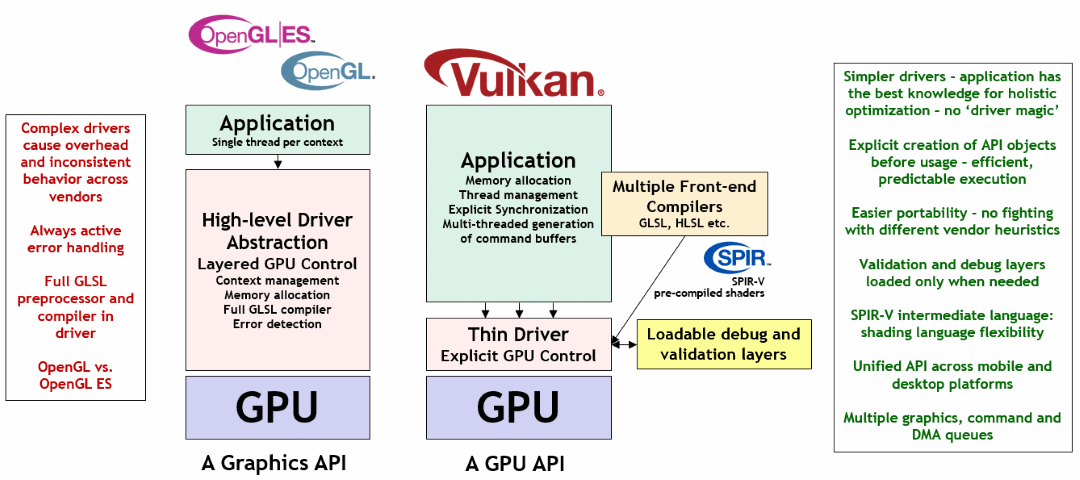
\includegraphics[width=\textwidth]{images/compare_opengl.png}
        \caption{OpenGL compared to Vulkan \citediagram{vulkan_guide}{1}.}
        \label{fig:compare_opengl}  
      \end{figure}

      While OpenGL acts as a state machine, keeping track of application state,
      Vulkan requires the developer to keep track of such state. OpenGL requires
      operations to be submitted in sequence, while Vulkan takes full advantage
      of modern multicore machines and allows operations to be recorded and
      submitted in parallel. \\

      OpenGL handles host-device synchronization and memory management in the
      driver, while Vulkan requires the developer to deal with this. The idea
      behind this is that the developer knows best how their data will be
      accessed and, as a result, the developer knows the optimal way to lay out
      data in memory. While this does result in a more explicit, low level API
      and longer development times, the advantage becomes apparent in the
      runtime speedup. There is much less overhead in the Vulkan driver, as the
      developer provides most of the required detail. Less driver work
      generally results in faster run times. \\

      OpenGL provides a constant level of error checking. While this is useful
      during the development phase, once an application is rolled out to
      production, error checking slows down the application. Vulkan provides
      a way around this with validation layers that can be registered during
      development and removed afterwards, further speeding up an application. \\

      OpenGL reads shader code in GLSL and compiles it at run time. This leads
      to a slower run time in the best case, or run time errors in the worst
      case when the GLSL is not properly formed. Vulkan requires the developer
      to compile the shader code to byte code (SPIR-V) ahead of time and to
      provide as such. This has the dual advantage of ensuring the shader
      code is correct and speeding up the run time. \\

      The pattern is apparent; Vulkan requires more setup, state tracking and
      memory management from the developer. This removes much of the required
      word from the driver, resulting in faster draw speeds in comparison
      with older APIs such as OpenGL.

    \section{Vulkan Layers}

      More traditional APIs have a flat structure. Any calls made to the API are
      forwarded to the driver for more work. If a developer wants to extend the
      structure and capabilities of the API, they are required to either "hack"
      together a platform-specific implementation, or have their extension
      built directly by the API developers into the API and driver. This
      increases the bulkiness of the API, requiring all users to have
      this large API when they may only use the minimal number of features.
      This "all-or-nothing" approach decreases the speed of the application,
      which is quite important for smaller applications running on embedded
      systems. \\

      Vulkan, in contrast, is a layered API, using a loader to create this
      layered architecture. This layered approach results in faster
      applications, as certain features which are needed in development,
      such as validation, can be unloaded when releasing an application.

      \subsection{Loader}

      The Vulkan loader is "the central arbiter in the Vulkan runtime" (TODO: quote).
      The application interfaces with the loader and it is the task of the
      loader to dispatch incoming requests to the correct subsystem. The
      loader exposes all of the core Vulkan functions. When an application
      calls such functions, they are routed through the loader, instead of
      directly to the driver. \\

      When creating an instance, certain extensions are required. Extensions
      are grouped into layers. These layers are specific to a system and
      platform and are registered in a well-known location on that machine
      in JSON files. These files contain the names of the extensions provided
      by the layer and where to find the actual library is on the system This
      means that whenever the Vulkan loader queries for a specific layer, the
      JSON file is read - the layer module itself does not need to be loaded. \\

      For example, a layer JSON file may be found at \\

      \begin{centering}
        \begin{Verbatim}[fontsize=\small]
/usr/local/share/vulkan/explicit_layer.d/VkLayer_khronos_validation.json
        \end{Verbatim}
      \end{centering}

      Included in the file may be the following (edited for brevity):

      \begin{centering}
        \begin{Verbatim}[fontsize=\small]
"instance_extensions": [
...
  {   
    "spec_version": "1", 
    "name": "VK_EXT_debug_utils"
  },
...
],
...
"library_path": "../../../lib/libVkLayer_khronos_validation.dylib"
        \end{Verbatim}
      \end{centering}


      \subsection{Dispatch Chains}

      A dispatch chain (figure \ref{fig:loader1}) is the path along which execution flows. The application
      calls a function, for example \verb|vkCreateInstance|. In the loader code, the
      layers and extensions are validated. The loader then passes execution
      along to the first layer, which also calls \verb|vkCreateInstance|, then
      passing execution along to the following layer. The loader terminates
      with its own code, before passing off the execution to the ICD
      (installable client driver). All available drivers are now combined
      into one unified front.

      \begin{figure}[h]
        \centering
        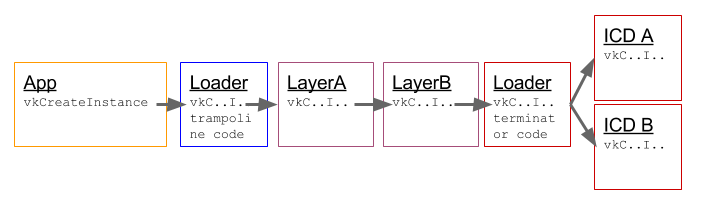
\includegraphics[width=\textwidth]{images/loader1.png}
        \caption{Vulkan dispatch chain \citediagram{renderdoc}{1}.}
        \label{fig:loader1}  
      \end{figure}

      This execution style also creates a dispatch table (figure \ref{fig:loader2}), where each layer in
      the queue calls \verb|vkGetInstanceProcAddr| on the next layer. This long
      chain of function pointers means that each layer knows how to pass on
      control to the next layer in the chain. 


      \begin{figure}[h]
        \centering
        \includegraphics[width=\textwidth]{images/loader2.png}
        \caption{Vulkan dispatch table \citediagram{renderdoc}{1}.}
        \label{fig:loader2}  
      \end{figure}

    \section{Vulkan Components}

      \begin{figure}[h]
        \centering
        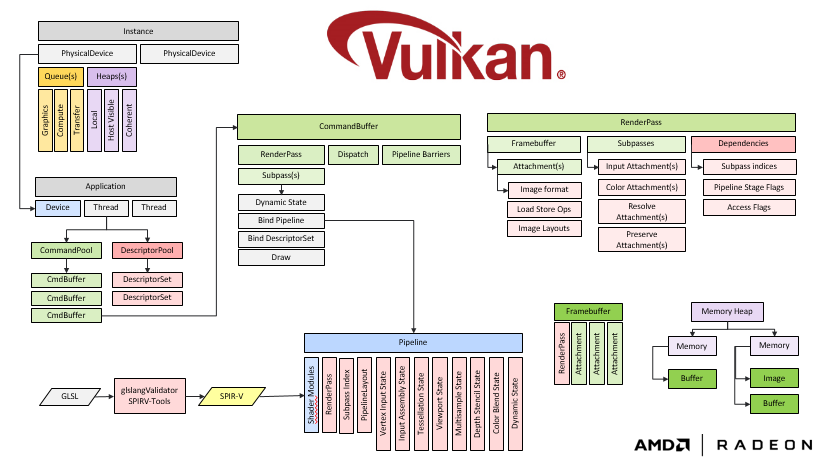
\includegraphics[width=\textwidth]{images/interactions.png}
        \caption{Vulkan API objects and their interactions \citediagram{vez}{1}.}
        \label{fig:interactions}  
      \end{figure}

      \subsection{VkInstance}
      
        A Vulkan instance is the first Vulkan component a developer creates in
        their application.  As Vulkan has no global state, all per-application
        state is contained within a Vulkan instance. By creating a VkInstance,
        the application loads the Vulkan commands and initializes Vulkan.
        Within each instance are multiple physical devices. \\

        After the Vulkan instance is created, devices and queues are the main
        way the application interacts with the Vulkan implementation.

      \subsection{VkPhysicalDevice}

        A physical device represents a single hardware device on the machine
        which has Vulkan capabilities, such as a GPU.

      \subsection{VkDevice}

        A logical device (simply a "device") is a software abstraction around a
        physical device. A physical device is queried for its capabilities and,
        based on required application criteria, a device is created from the
        suitable physical device. A device represents an instance of a
        physical device and contains its own state and resources. This is
        the Vulkan component that is most commonly interacted with and is
        used in constructing all subsequent components. An application is
        required to create a different device for each physical device it uses.
        Each device exposes a number of queues.

      \subsection{VkQueue}

        A queue is where a piece of work is submitted for completion by the GPU,
        for example a draw command. A queue is created in conjunction with a
        device and the application queries the device for a suitable queue.
        Queues are partitioned into a set of families, where each family
        supports one or more types of functionality. Examples of such
        functionality include graphics, presentation and compute. For most
        applications, graphics functionality is required to modify the
        incoming vertices and presentation support is required to display
        the resulting images on the screen. 

        Queue submission occurs when work is submitted to a queue using commands
        such as vkQueueSubmit. Such commands specify a set of underlying
        operations which are to be executed by the associated physical
        device. 

        Each queue works asynchronously to other queues, making it suitable for
        multithreaded use.

      \subsection{VkDeviceMemory}

        Memory is explicitly managed by the application. There are two types of
        memory in Vulkan, host memory and device memory. Device local memory is
        physically connected to the device, while host visible memory is
        visible to the host. Each device exposes the types of memory available
        to the application. \\

        When creating a buffer, the user must specify both how the buffer will
        be used and where this buffer will reside. Host-visible memory can be
        accessible by the CPU through the use of the vkMapMemory command, while
        the device-local is the most efficient for GPU access.

      \subsection{VkCommandBuffer}

        The application can control the device through the submission of command
        buffers. Prior to submission, the application records units of work
        into these command buffers. These command buffers may be constructed
        over multiple threads and may be reused multiple times. The command
        buffers are submitted to queues. Command buffers in separate queues
        may execute in parallel, while command buffers in a single queue
        execute in respect to queue submission order. Upon command buffer
        queue submission, control is returned to the application immediately. \\

        There are two different types of command buffers,
        primary command buffers and secondary command buffers.

        \begin{itemize}
          \item A primary command buffer is submitted to a queue for execution.
          It holds references to an array of secondary command buffers.
          \item A secondary command buffer is not submitted to a queue for
          execution. Instead, work is recorded into it and a reference to the
          command buffer is attached to a primary command buffer, along with
          other secondary command buffers. This allows for multiple threads to
          construct multiple secondary command buffers in parallel, attach
          them to a primary command buffer and submit for execution.
        \end{itemize}

        All of this work can be recorded into the buffers ahead of draw time,
        resulting in faster draw speeds.

      \subsection{VkSwapchainKHR}

      %TODO

    \section{Vulkan Object Model}

      Vulkan objects (VkInstance, VkDevice and so on) are represented by
      handles - an abstract reference to a piece of memory that is managed by
      Vulkan. Handles come in two types; dispatchable and non-dispatchable.

      Dispatchable objects consist of a pointer to an opaque type. These
      objects internally hold a dispatch table. This table is used by other
      components of the system to determine what code to execute when the
      application makes calls to Vulkan. Examples of dispatchable objects
      include the VkInstance, VkPhysicalDevice, VkDevice, VkCommandBuffer
      and VkQueue. The first argument to any Vulkan function is a
      dispatchable object. This excludes VkInstance creation, as this
      is the first dispatchable Vulkan object created.

      Non-dispatchable objects are 64-bit integer types which are
      implementation dependent. They either contain a reference to another
      object, or encode information about the object directly. Objects
      created on a specific device are private to that device and cannot
      be used on another device.

  \chapter{The evulkan Library}

    \section{How does it work?}

      The library exposes a number of components, each of which is a wrapper
      around one or more Vulkan objects.

      \subsection{evk::Device}

        A device is the basic component of the library. It is the first Vulkan
        component that is constructed in the application. It encapsulates,
        among other things, a VkInstance, VkPhysicalDevice, VkDevice, VkQueues.
        A user can set up the device with or without validation layers. Leaving
        validation layers turned off results in a faster application suitable
        for production. \\

        The Device object tracks state across the program. It is used in the
        creation of other evk Vulkan objects. The Device is responsible for
        creating a VkInstance, VkPhysicalDevice, VkDevice, VkSwapchainKHR, VkFramebuffer
        and all the required command buffers. \\

        The Device is multithreaded, making use of Vulkan's multithreading
        capabilities. For some more intensive operations, such as recording
        draw operations into the command buffer, it splits the operation
        across multiple threads, each of which records its portion of the
        operation into a separate secondary command buffer. \\

        \begin{figure}[h]
        \begin{verbatim}
            vkCmdDrawIndexed(
              secondaryCommandBuffer, numIndices,
              1, indexOffset, 0, 0
            );
        \end{verbatim}
        \end{figure}

        These secondary command buffers are then executed from the primary
        command buffer.

        \begin{figure}[h]
        \begin{verbatim}
            vkCmdExecuteCommands(
              primaryCommandBuffer,
              secondaryCommandBuffers.size(),
              secondaryCommandBuffers.data()
            );
        \end{verbatim}
        \end{figure}

        \begin{wrapfigure}{l}{\figurewidth}
          \centering
          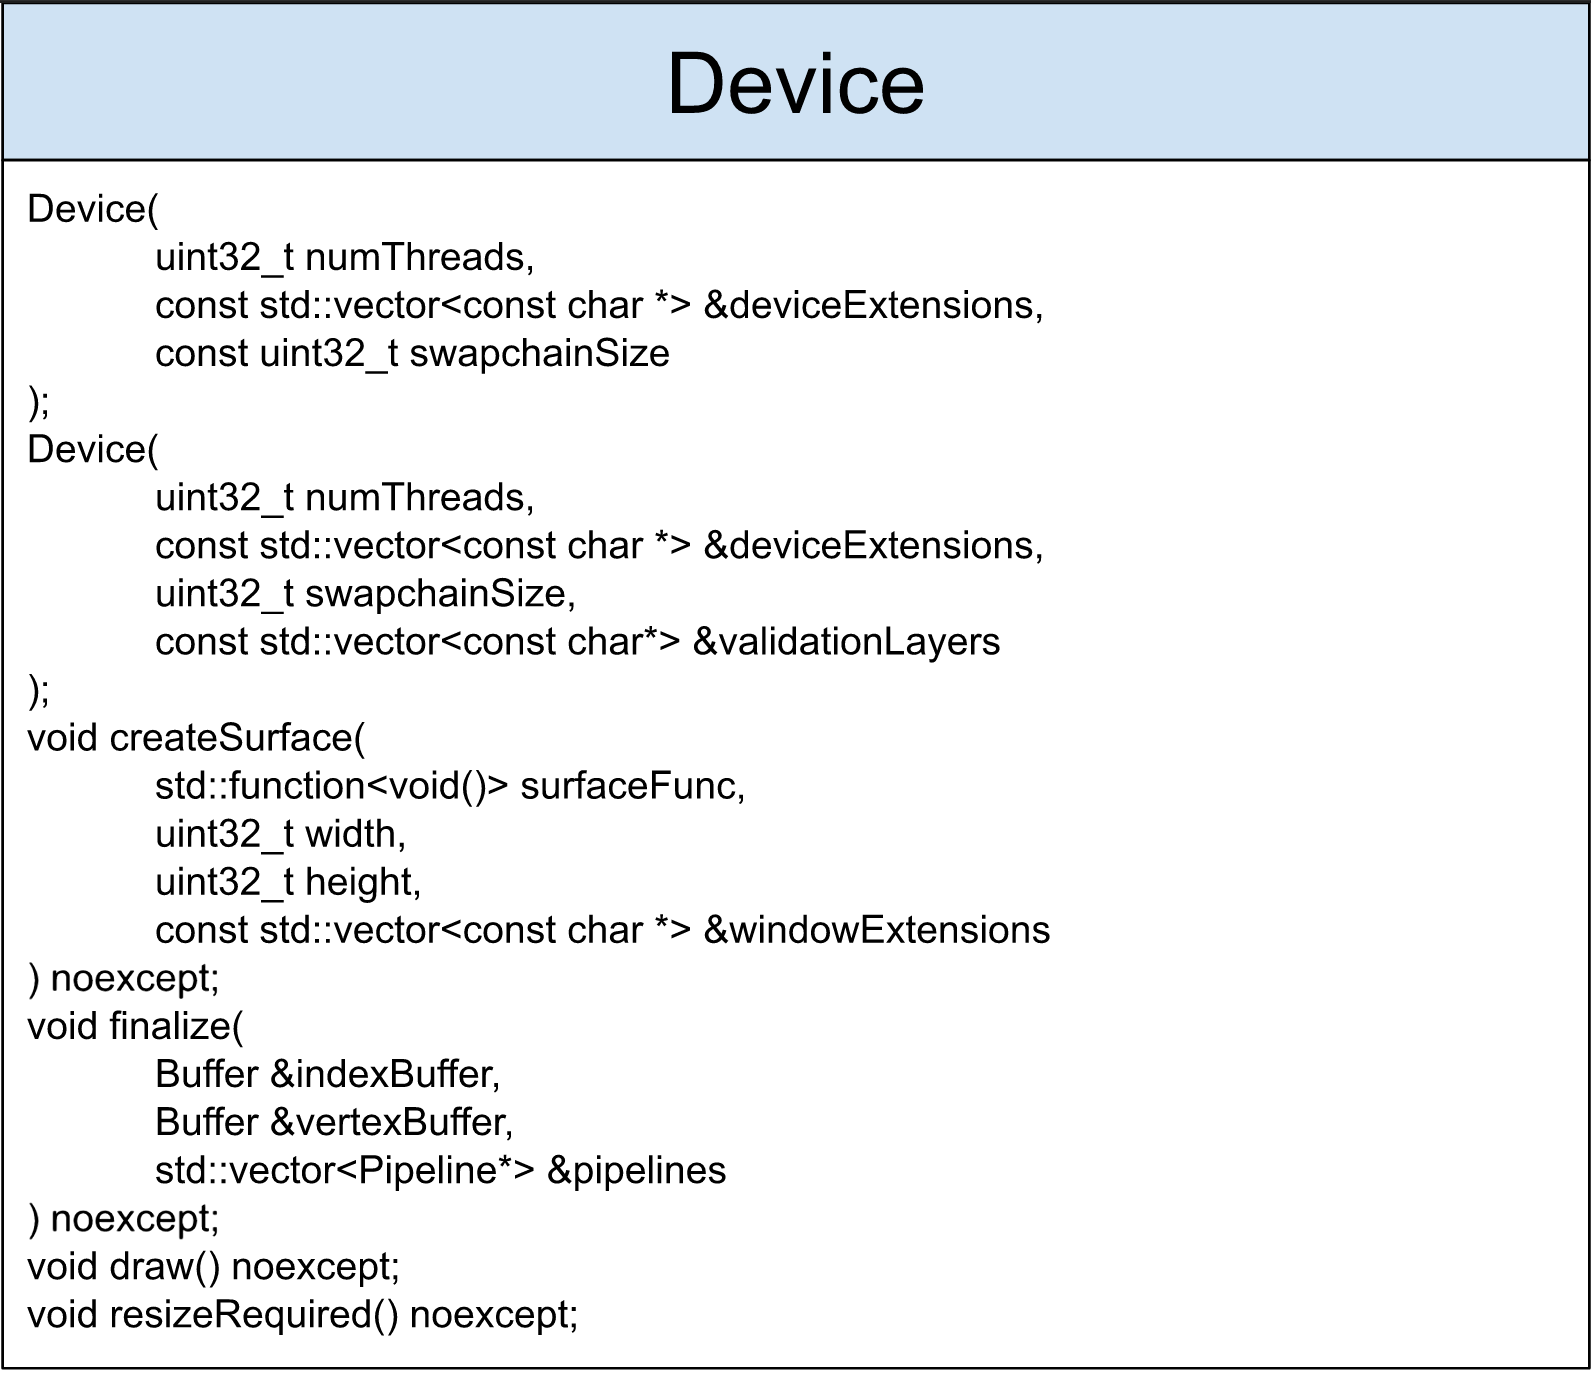
\includegraphics[width=\imagewidth]{images/class_device.png}
          \caption{Device class diagram.}
          \label{fig:class_device}  
        \end{wrapfigure}

      \subsection{evk::Texture}

        \begin{wrapfigure}{l}{\figurewidth}
          \centering
          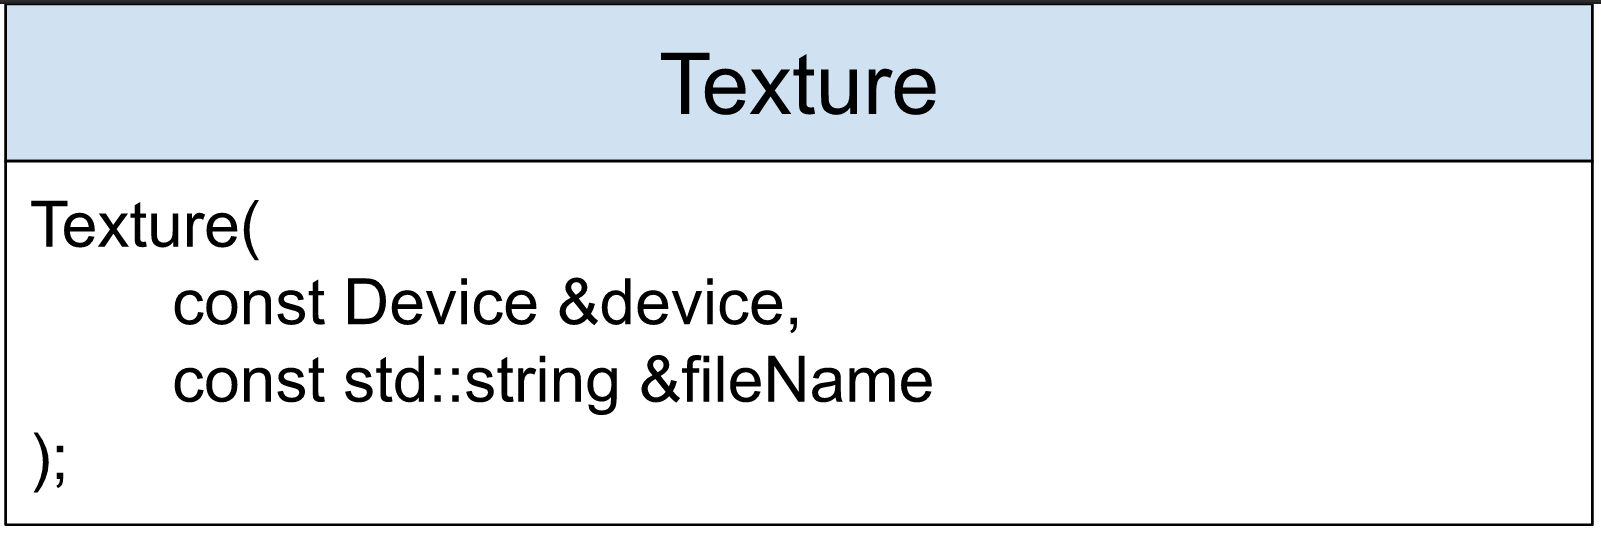
\includegraphics[width=\imagewidth]{images/class_texture.png}
          \caption{Texture class diagram.}
          \label{fig:class_texture}  
        \end{wrapfigure}

      \subsection{evk::Attachment}

        \begin{wrapfigure}{l}{\figurewidth}
          \centering
          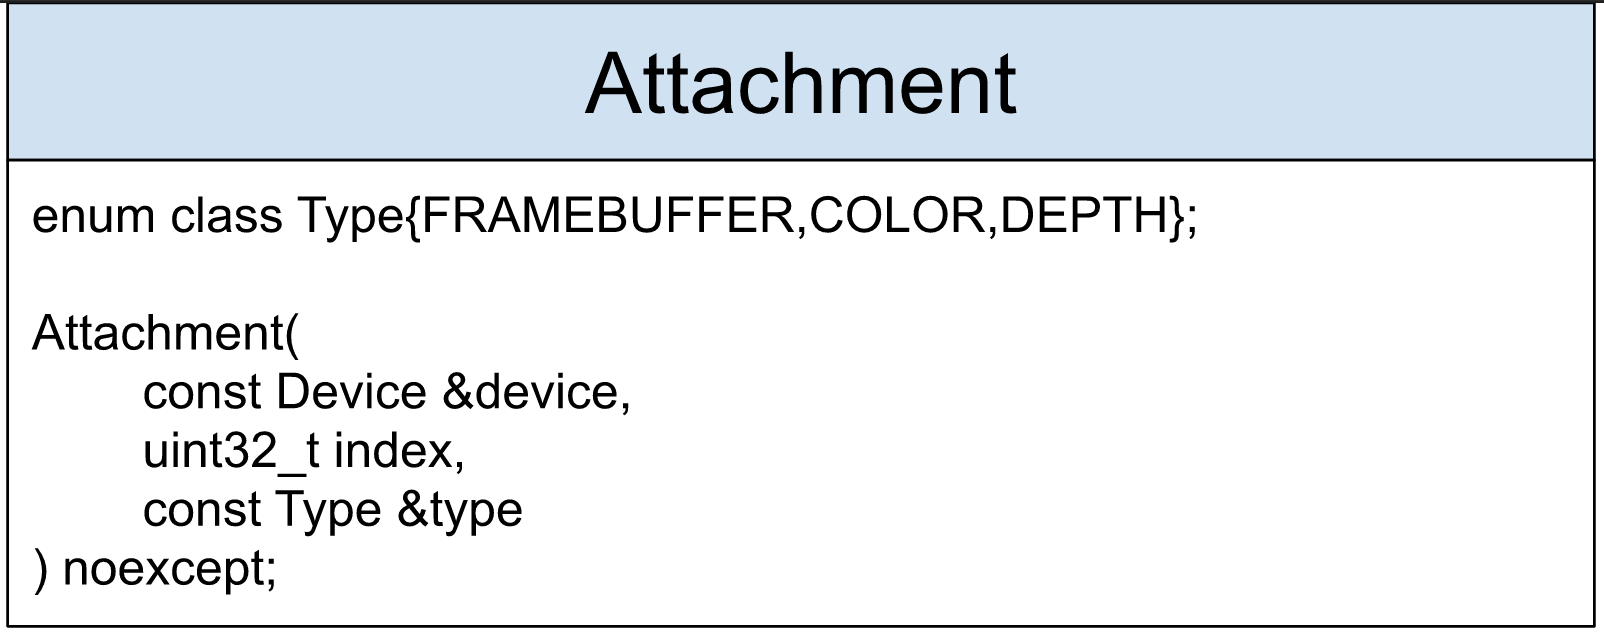
\includegraphics[width=\imagewidth]{images/class_attachment.png}
          \caption{Attachment class diagram.}
          \label{fig:class_attachment}  
        \end{wrapfigure}

  \begin{wrapfigure}{l}{\figurewidth}
    \centering
    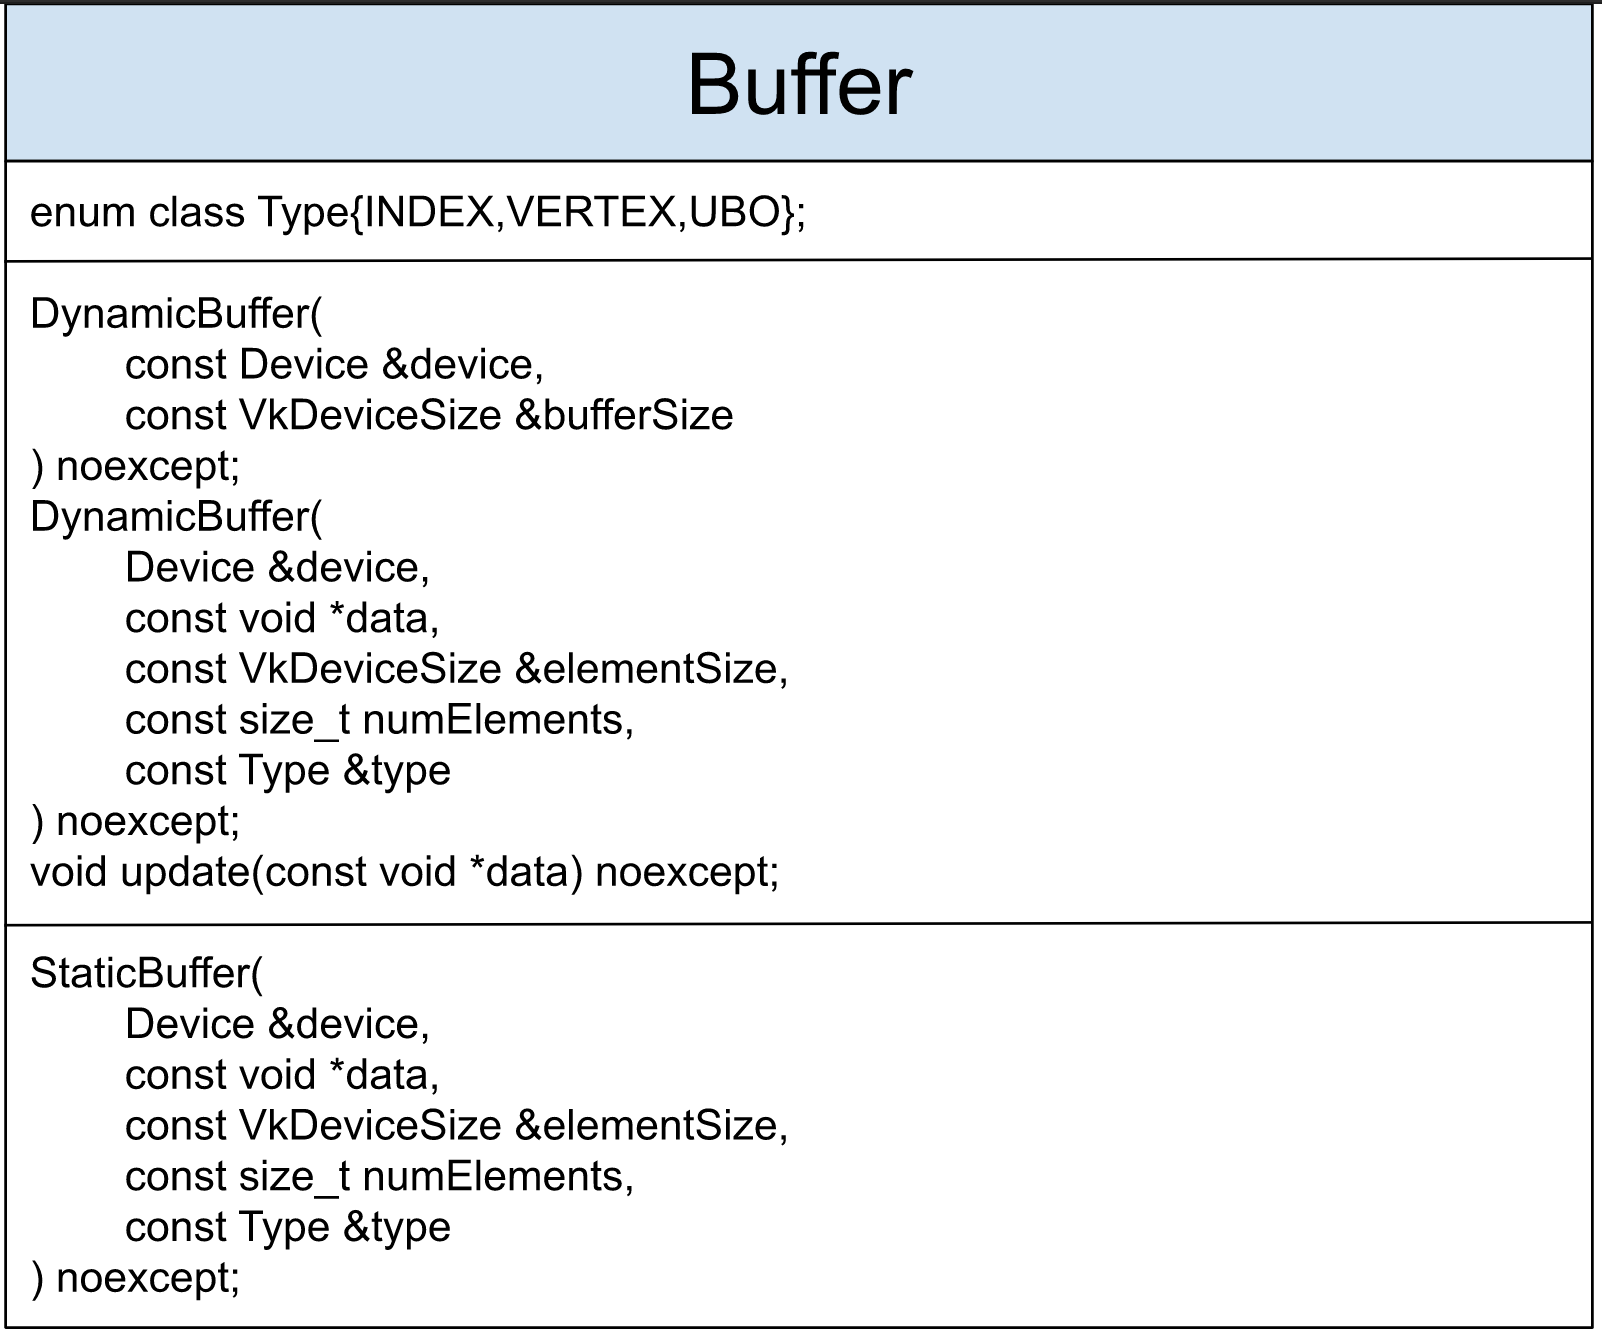
\includegraphics[width=\imagewidth]{images/class_buffer.png}
    \caption{Buffer class diagram.}
    \label{fig:class_buffer}  
  \end{wrapfigure}

  \begin{wrapfigure}{l}{\figurewidth}
    \centering
    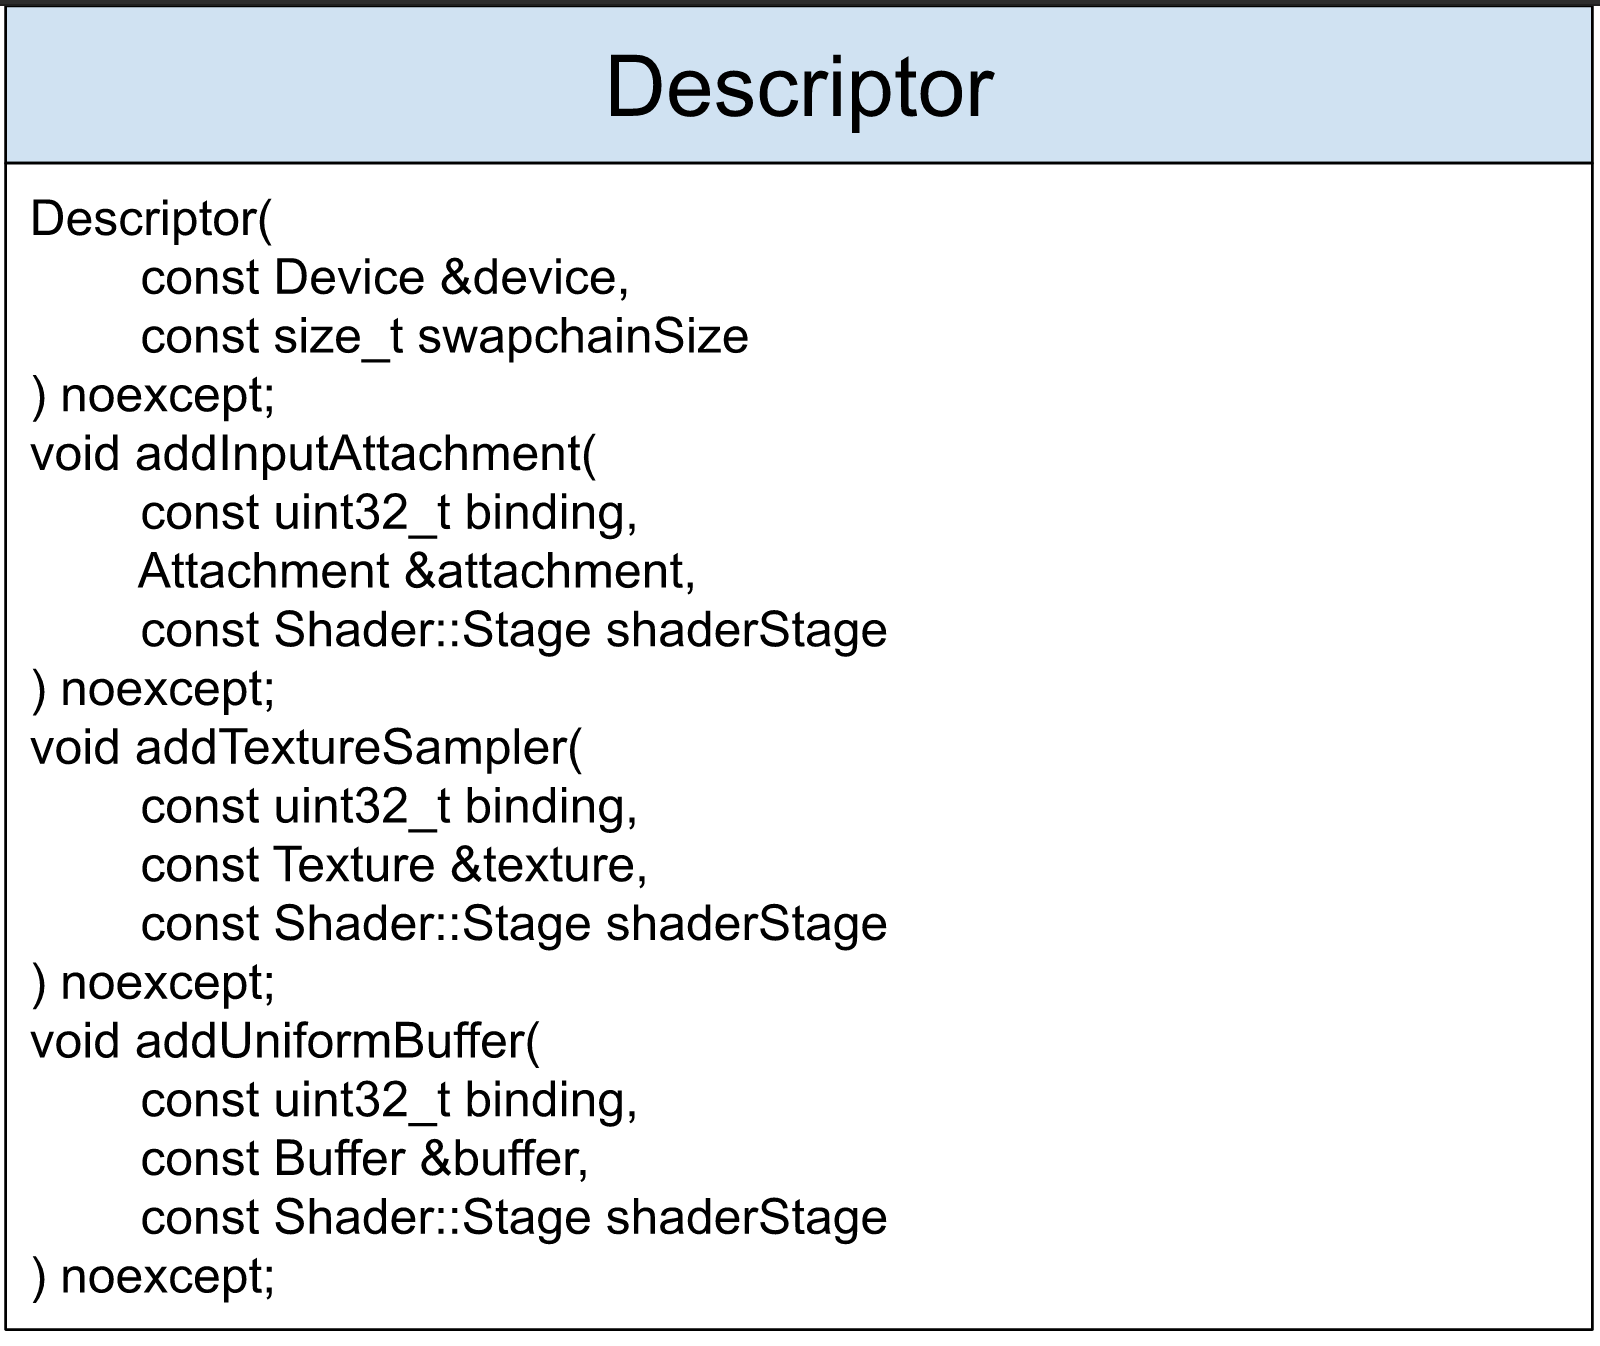
\includegraphics[width=\imagewidth]{images/class_descriptor.png}
    \caption{Descriptor class diagram.}
    \label{fig:class_descriptor}
  \end{wrapfigure}

  \begin{wrapfigure}{l}{\figurewidth}
    \centering
    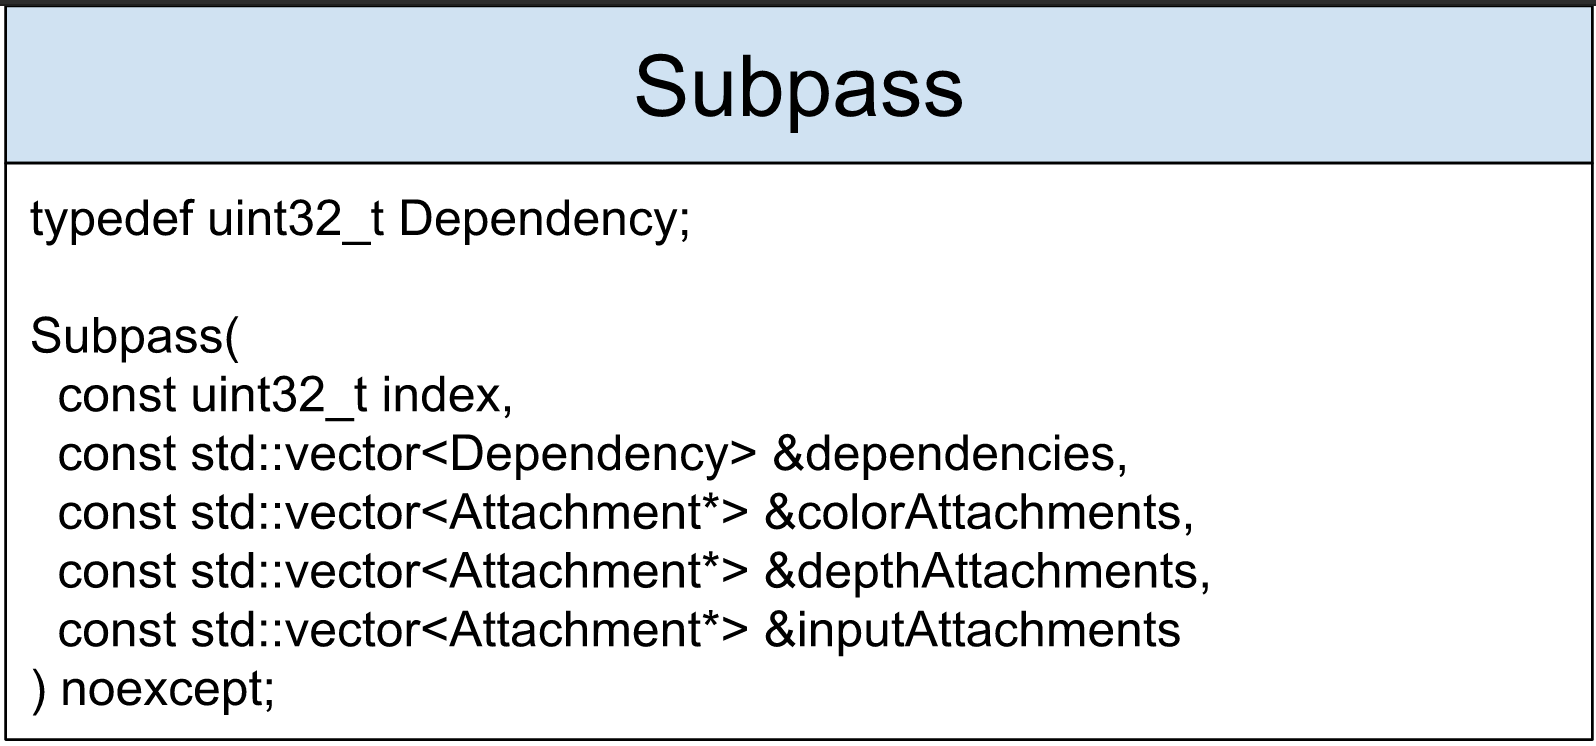
\includegraphics[width=\imagewidth]{images/class_subpass.png}
    \caption{Subpass class diagram.}
    \label{fig:class_subpass}
  \end{wrapfigure}

  \begin{wrapfigure}{l}{\figurewidth}
    \centering
    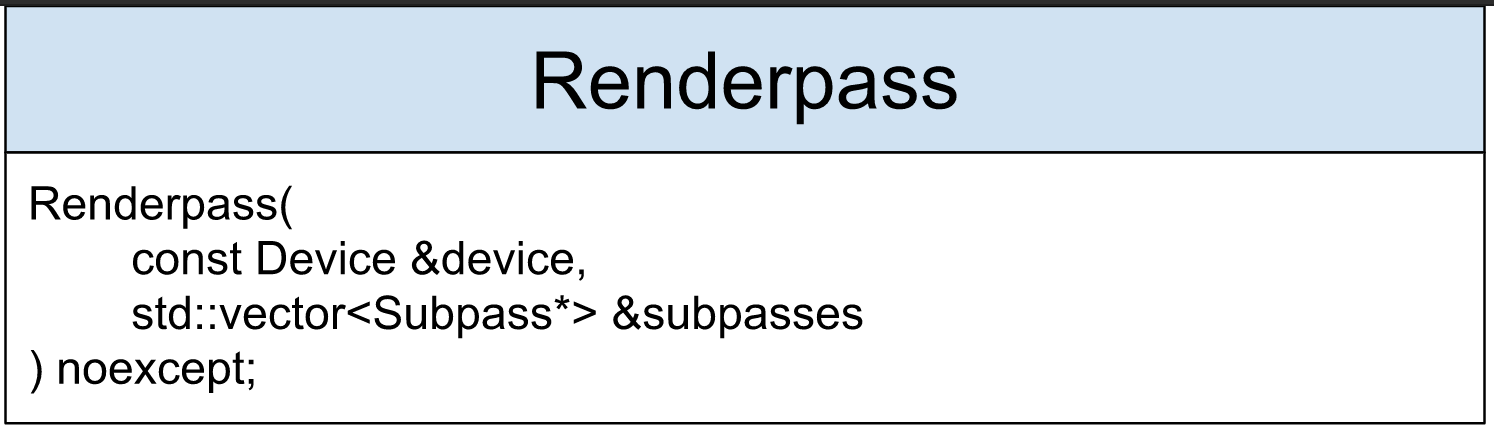
\includegraphics[width=\imagewidth]{images/class_renderpass.png}
    \caption{Renderpass class diagram.}
    \label{fig:class_renderpass}
  \end{wrapfigure}

  \begin{wrapfigure}{l}{\figurewidth}
    \centering
    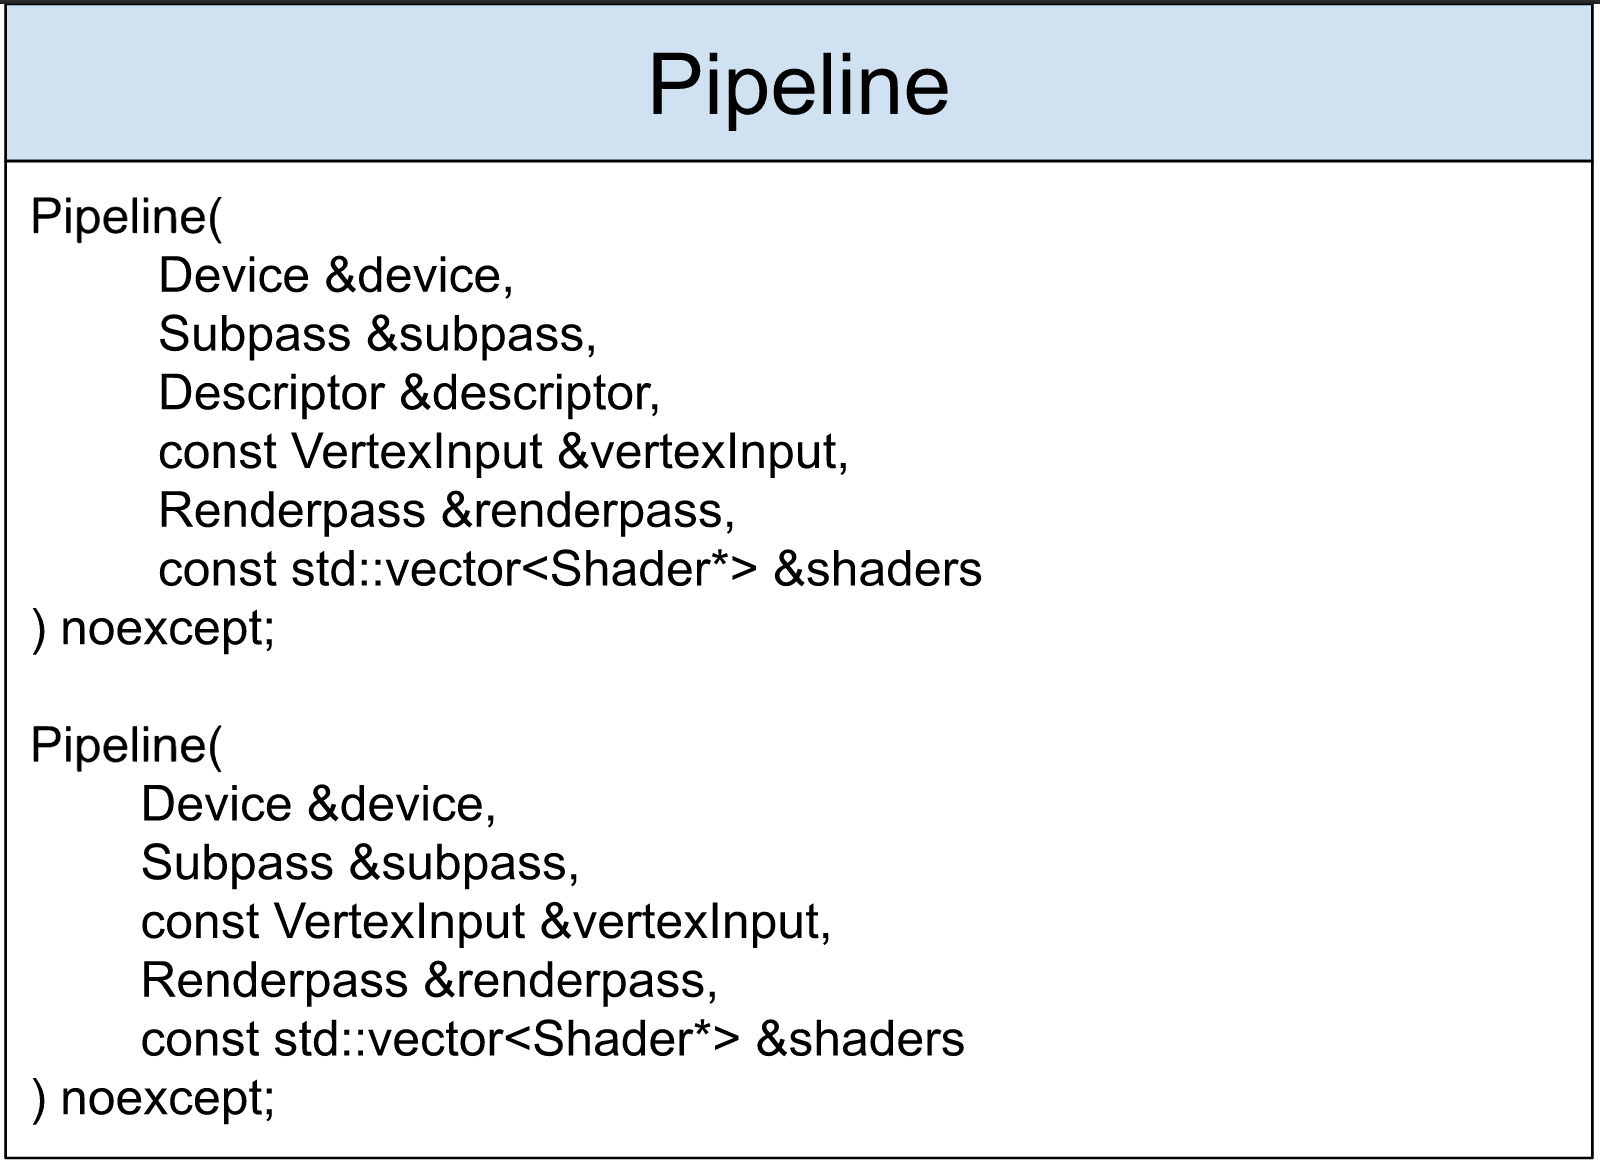
\includegraphics[width=\imagewidth]{images/class_pipeline.png}
    \caption{Pipeline class diagram.}
    \label{fig:class_pipeline}
  \end{wrapfigure}

  \begin{wrapfigure}{l}{\figurewidth}
    \centering
    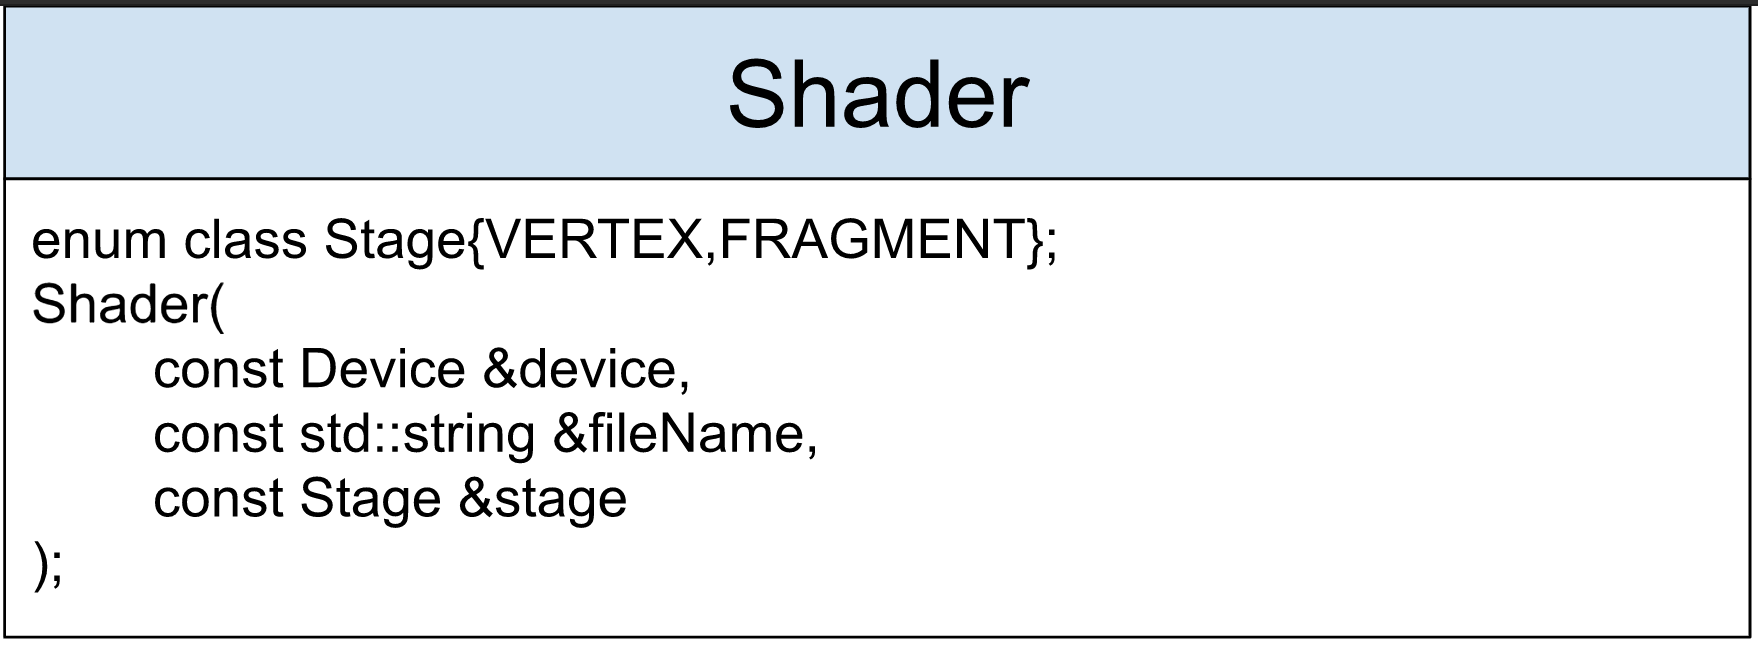
\includegraphics[width=\imagewidth]{images/class_shader.png}
    \caption{Shader class diagram.}
    \label{fig:class_shader}
  \end{wrapfigure}

  \begin{wrapfigure}{l}{\figurewidth}
    \centering
    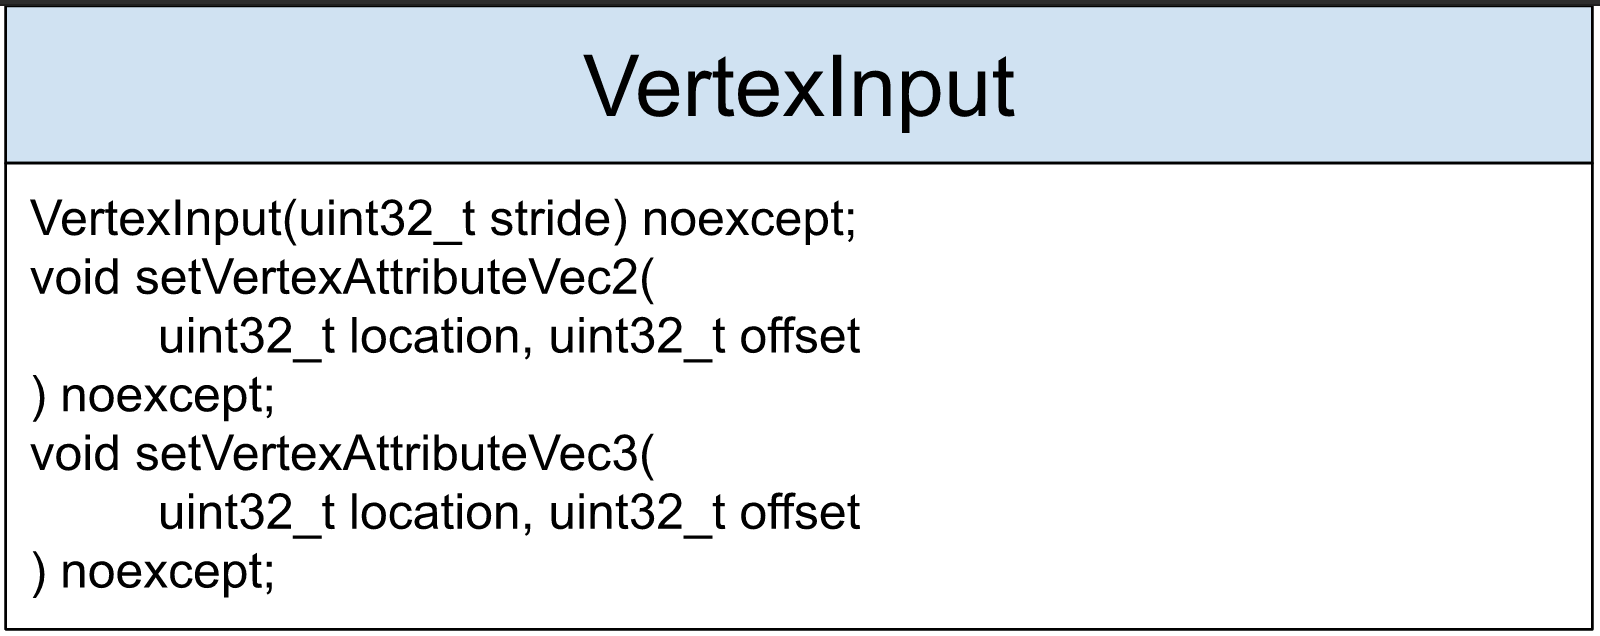
\includegraphics[width=\imagewidth]{images/class_vertexinput.png}
    \caption{VertexInput class diagram.}
    \label{fig:class_vertexinput}
  \end{wrapfigure}

  \begin{figure}[h]
    \centering
    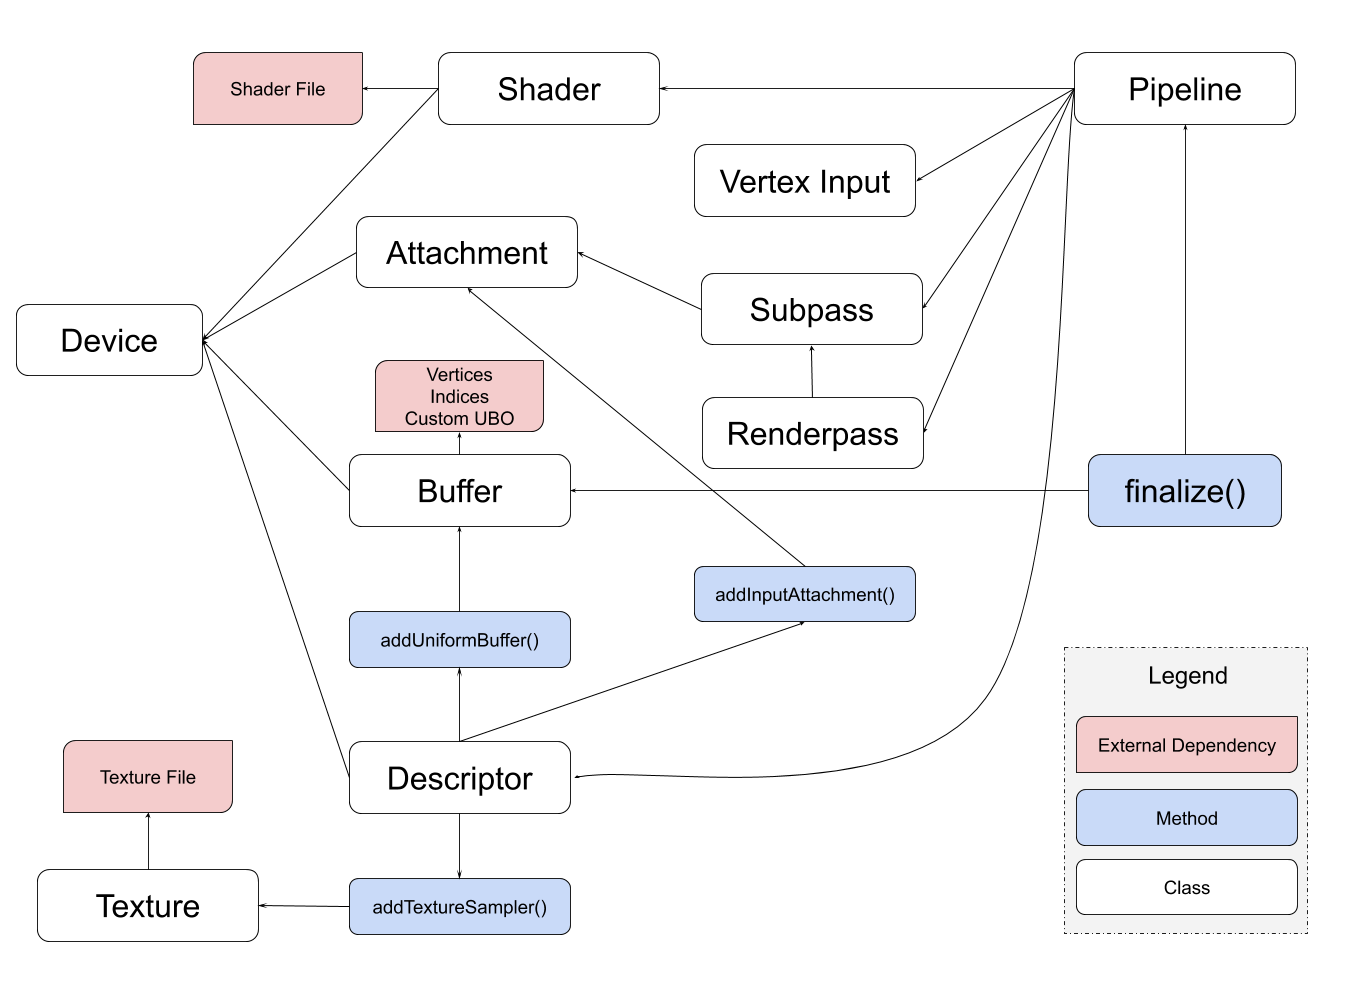
\includegraphics[width=\textwidth]{images/evk_architecture.png}
    \caption{evulkan architecture.}
    \label{fig:evulkan_architecture}  
  \end{figure}

  \chapter{Conclusion}

  \afterpage
  {
    \begin{figure}
      \begin{subfigure}[b]{\textwidth}
        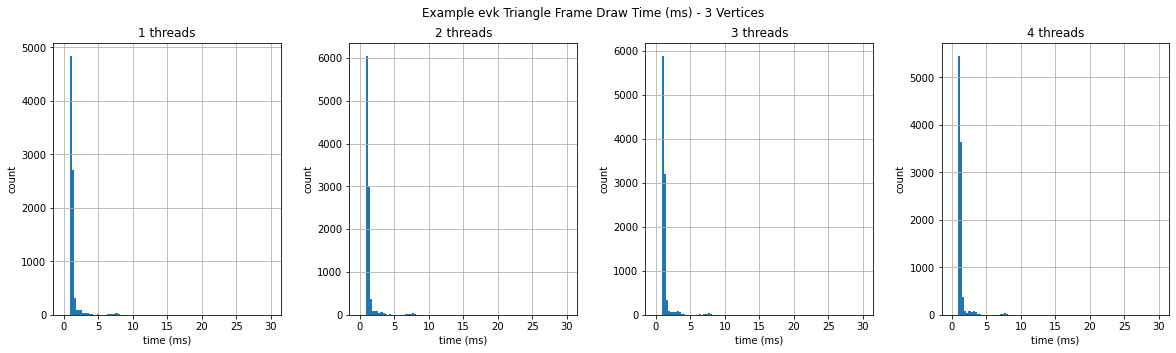
\includegraphics[width=\textwidth]{images/triangle_draw.png}
      \end{subfigure}
      \begin{subfigure}[b]{\textwidth}
        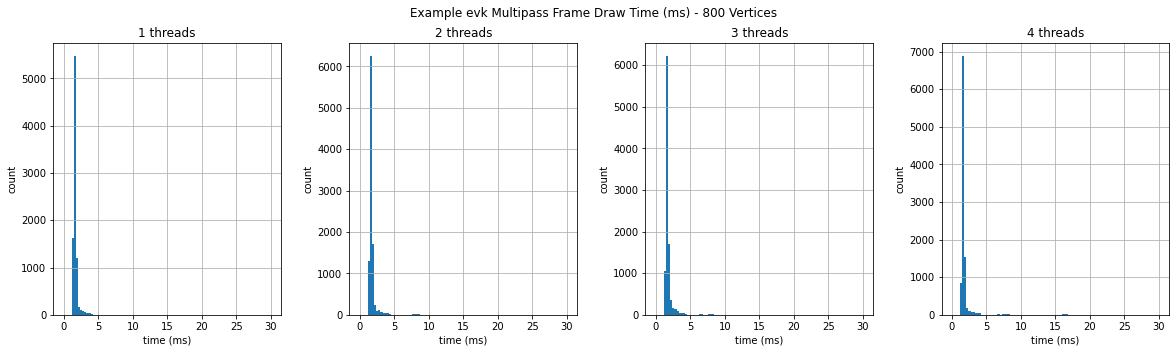
\includegraphics[width=\textwidth]{images/multipass_draw.png}
      \end{subfigure}
      \begin{subfigure}[b]{\textwidth}
        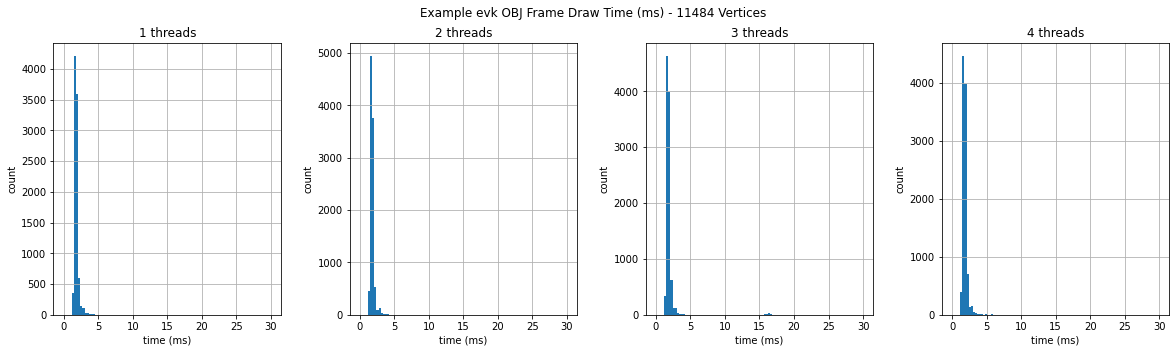
\includegraphics[width=\textwidth]{images/obj_draw.png}
      \end{subfigure}
      \caption{Draw time for different examples over multiple threads.}
      \label{fig:draw}                        
    \end{figure}

    \clearpage

    \begin{figure}
      \begin{subfigure}[b]{\textwidth}
        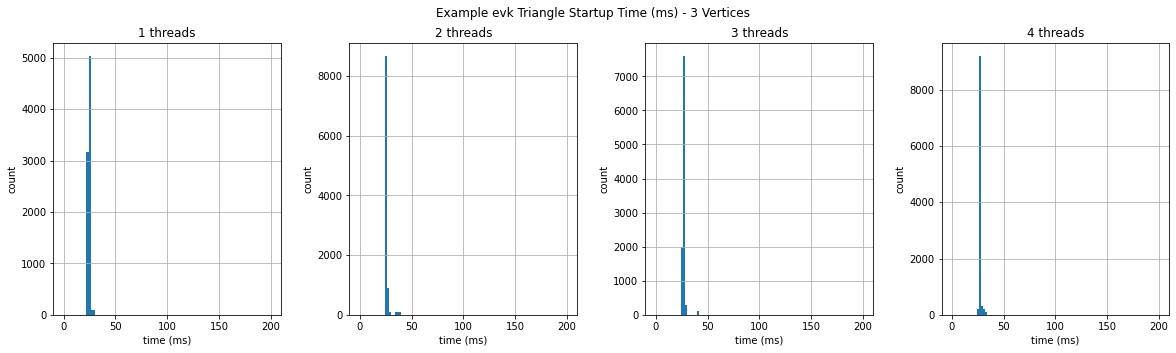
\includegraphics[width=\textwidth]{images/triangle_setup.png}
      \end{subfigure}
      \begin{subfigure}[b]{\textwidth}
        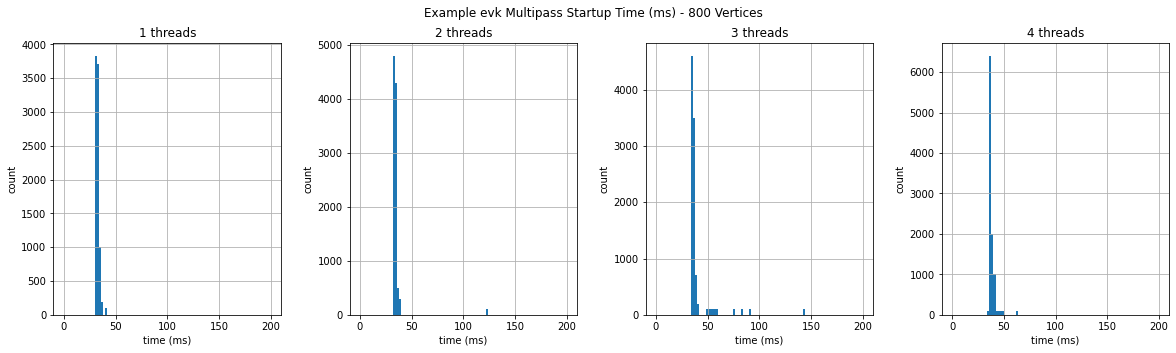
\includegraphics[width=\textwidth]{images/multipass_setup.png}
      \end{subfigure}
      \begin{subfigure}[b]{\textwidth}
        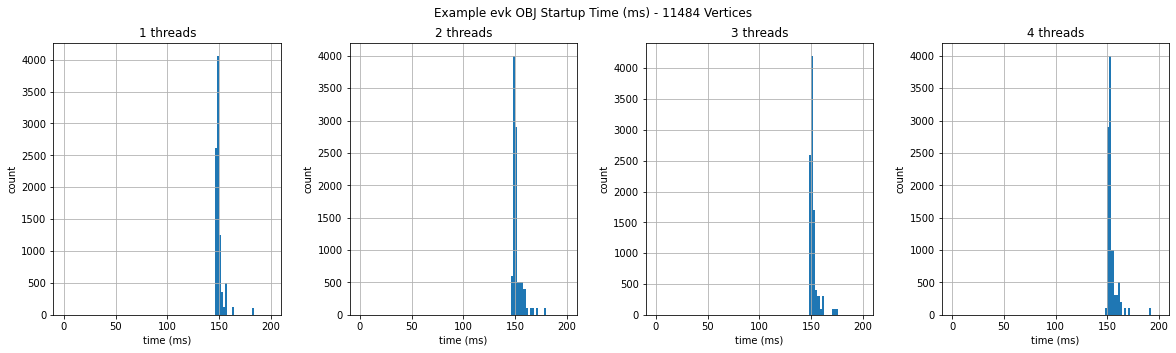
\includegraphics[width=\textwidth]{images/obj_setup.png}
      \end{subfigure}
      \caption{Setup time for different examples over multiple threads.}
      \label{fig:setup}                        
    \end{figure}
    
    \clearpage
  }

  \bibliographystyle{harvardnat}
  \bibliography{thesis.bib}

  \chapter*{Appendices}
  
\end{document}